\documentclass[12pt,a4paper]{article}

\usepackage{geometry}
\geometry{margin=1in}
\usepackage{titlesec}
\usepackage{graphicx}
\usepackage{amsmath}
\usepackage{hyperref}

\title{Literature Review \\ \large An Algorithmic Approach to Route Planning for Cyclists}
\author{Jack Jibb \\ MSc Computer Science}
\date{\today}

\begin{document}

\maketitle

\tableofcontents
\newpage

\section{Categorization and Separation Algorithm Design and Analysis}

\subsection{Research Objectives}
The purpose of creating an algorithmic approach to categorizing and segmenting a GPX route is to be able to rapidly and systematically construct new routes based on the requirements of the rider's training plan.
It makes sense intuitively to segment a route, so riders does not have to analyse every part of a map to determine where to send their route. Riders are specifically interested in sections of the route such as climbs, descents, busy roads, and gravel.
The objective of research should be to come up with a suitable method of segmentation, and subsequent categorization of the resulting segments so riders can select ones that suit their training needs.
\\
In order to achieve the categorization, it is necessary to know what athletes require for training. This is a complex topic with a lot of nuance, however as far as route planning goes, cyclists mostly look for six main factors.
Here are the main actions that need to be considered:
\begin{itemize}
	\item \textbf{Segmentation-by-road-name} - The simplest separation, if the name of the road changes (i.e. at an intersection)
	\item \textbf{Categorization-by-road-type} - If the surface of the road, or the road purpose changes (bike lane, shared use, gravel, etc)
	\item \textbf{Categorization-by-gradient} - If a significant hill occurs (+/- 4\% sustained for at least 500m)
	\item \textbf{Categorization-by-road-width} - If the width of a road becomes larger or smaller suddenly (changing from dual to single lane, road-side parking, etc)
	\item \textbf{Categorization-by-sharp-turn} - If a road suddenly has a sharp bend
	\item \textbf{Categorization-by-road-behaviour} - If a road becomes twisty, or enters a forest or village.
\end{itemize}

\subsection{Algorithmic Approaches to Segmentation and Categorization}
There are several methdologies when it comes to segmentation, including (but not limited to) clustering, heuristic methods, signal analysis, and map-based segmentation. Some, or all of these may be
applied to the algorithm, since there is not one method to solve all segmentation types. What follows is a review of the literature that exists that could contribute to
achieving advanced segmentation.


\paragraph{Paul Newson and John Krumm: "Hidden Markov Map Matchign Through Noise and Sparseness"}
A useful way to clean up the location data as a pre-processing step could be through map matching. Newson and Krumm explore map-snapping through a HMM model on timestamp-marked latitude and longitude pairs.
The approach showcased in the paper is focused on automobile traffic, so there may be some need to tweak the emission delta for bikes, to accomodate for larger variance in the horizontal travel distance, as well as increasing
the search range for nodes around each track point. The search would then use a Gaussian probability curve, centred on GPX trackpoint, with nodes closer being more likely than ones further away. Then a transition probability will be implemented between consecutive points
so straight line distance is more probable. Lastly, a Viterbi algorithm will be run to find the "most likely" node sequence.
Once the node sequence is determined, the sequence of ways can then be determined.

\paragraph{Wang et al., “CycleTrajectory: An End-to-End Framework for Enriching Cycling Trajectory Data”}
The authors propose a framework to provide a pipeline to correct GPS data with OpenStreetMap metadata for cycling behaviour analysis. This allows
OSM tags to be implemented into each trajectory point. This provides a fully automated and open source method for implementing OpenStreetMap data to any file that contains Latitude and Longitude points.
It also allows for a smarter noise reduction method than a simple low pass filter. Some downsides however, are that it is dependent on OSM coverage, as well as snapping errors in dense urban areas due to proximity of roads. It also relies on consistent naming and mapping schemes, when
in reality, as the data is sourced globally, not all data features will be correctly labelled or formatted.

\paragraph{Evgeny Arbatov: "GPX Route Generator"}
Arbatov provides a self-contained route planner that can take two endpoints, and plot a route between them, prioritising the shortest, but also allowing for preference, for example, preferring park-connector routes.
The application is written in Lua and is run in docker-compose. The work here provides a simple weighting mechanic, but could be useful when it comes to segmentation.
They use OSM's nearest-node API to pull intersection nodes, and generate a track from the connected ways. This means segments could be generated automatically from finding waypoints, a method for segmentation-by-road-name

\paragraph{Boeing, G: "Modeling and Analyzing Urban Networks and Amenities with OSMnx"}
Boeing Details a novel Python package that downloads and analyses street networks from OpenStreetMap, which implements simple query langauge for pulling street data from the OSM database. It also includes tools for simplifying OSM map data so
ways and nodes represent roads and intersections, which is useful for cleaning up a network created by the CyclingTrajectory framework. It is important to note however that by reducing the map's complexity, it does increase computational complexity, so there is a trade-off there.



\subsection{Applications in Cyclist Route Planning}
% How segmentation algorithms are applied in training route selection and analysis
In the creation of a route, segmentation should be done automatically if a segment doesn't already exist in the database. Additionally, each route should be converted to
a series of OSM ways, for purpose of generating a Training Suitability Score.

\subsection{Methodological Considerations and Assumptions}
\begin{itemize}
	\item Filtering of route signal to reduce noise
	\item Tuning the algorithms manually may be required to best align the segmentation strength.
\end{itemize}
\newpage

\section{Training Suitability Scoring Methodologies}

\subsection{Research Objectives}
Implementing a summative score that represents a section requires access to rider metrics, GPS data, and historical data. This is more an art than a science, and requires
experience in cycling lots of roads, but also can be boiled down to six main metrics:
\begin{enumerate}
	\item Safety (a composite metric defined by various factors, could also be gathered collectively from rider feedback)
	\item Difference between Average and Normalized Power
	\item Length (of segment)
	\item Elevation Gain (or loss)
	\item Road Surface Quality
	\item Absolute Normal Distance Change (aka how twisty the road is)
\end{enumerate}


\subsection{Approaches to Suitability Scoring}

\paragraph{Sharifzadeh et al. "Change Detection in Time Series Data Using Wavelet Footprints"}
An interesting approach to Suitability scoring relates to Fast Fourier Transforms, and a convolution approach comes from Medhi Sharifzadeh et al, from the University of Southern California, introducing a concept known as
"wavelet footprints" as a compact, multi-resolution approach to representation of spatial-temporal trajectories. Wavelet footprints are a  more granular version of the Wavelet Transform, which in turn is a version of the Fourier Transform. The approach involves using Wavelets to transform a signal into the "Wavelet Domain".
The smaller the wavelet, the more reactive it will be to change in the original signal, so by adjusting the size of the wavelet, the signal can be filtered to be more or less reactive to change.
Wavelet footprints have an advantage over the general Wavelet transform, where they only retain the most significant components. This is done by having wavelets occur in orthoganal sets.
Due to Heisenberg's Uncertainty Principle, it is impossible to perfectly describe both the frequency content of a signal and the location in time of the signal. Time-domain and Frequency-Domain analysis in this regard are
at opposite ends of the spectrum, but the Wavelet Domain sits in the middle, allowing for a sliding scale value, where a larger scale gives more frequency and less time resolution, while smaller scales give less frequency, and more time resolution.
The following are some key concepts from the paper that will be useful in implementation of the algorithm:

\begin{itemize}
	\item \textbf{Wavelet Decomposition of Trajectory}: \\ Given a signal $x[n]$ of length $N$, it can be expressed as a wavelet series:
	      \[
		      x[n] =
		      \sum_{j=0}^{J-1} \sum_{k} d_{j,k} \, \psi_{j,k}[n]
		      + \sum_{k} c_{J,k} \, \phi_{J,k}[n]
	      \]
	      where:
	      \begin{itemize}
		      \item $\psi_{j,k}[n]$ are the wavelet basis functions at scale $j$ and position $k$.
		      \item $\phi_{J,k}[n]$ are the scaling functions at the coarsest level $J$.
		      \item $d_{j,k}$ are detail coefficients at scale $j$ and position $k$.
		      \item $c_{J,k}$ are approximation coefficients.
	      \end{itemize}
	\item \textbf{Footprint Definition}\\
	      The \textbf{wavelet footprint} of $x$ is defined as the set of significant coefficients:
	      \[
		      F(x) = \{ (j,k) \;|\; |d_{j,k}| > T_j \}
	      \]
	      where $T_j$ is a scale-dependent threshold, which can be tuned to correspond to physiological thresholds of training intensity zones. This is useful since
	      at different scales, the detail coefficients are not comparable, so the threshold must be defined explicitly.

	\item \textbf{Footprint Calculation}\\
	      To calculate the Wavelet Footprint, first the detail coefficient, $d_{j,k}$ is extracted. Since not all detail coefficients are meaningful, a scale-dependent threshold $T_j$
	      is defined to filter out noise. This is calculated with the standard deviation of the specific scale:
	      \[
		      T_j = \gamma_j \dot \sigma_j
	      \]

	      Where:
	      \begin{itemize}
		      \item $\sigma_j$ is the standard deviation of $d_{j,k}$ at scale $j$.
		      \item $\gamma_j$ is the tuning parameter.
	      \end{itemize}
	      This value can then be used to define the Footprint Definition described earlier.

	\item \textbf{Compact Representation}\\
	      To reduce dimensionality, only the $k$ largest coefficients can be retained:
	      \[
		      F_k(x) = \text{top-}k \text{ elements of } F(x)
	      \]
	      This is useful to optimize data set size, while not reducing the accuracy of the data significantly.
	\item \textbf{Matching and Distance}\\
	      The overall difference in two signals $x$ and $y$ can be approximated by taking the difference of their footprints:
	      \[
		      D(x,y) \approx \| F(x) - F(y) \|
	      \]

\end{itemize}

The advantage of using wavelet footprints over the Fourier Transform means that it is possible to isolate points in the signal where significant changes occur in specific metrics, or combination of metrics, allowing flexibility in choosing
what conditions must be met to enact a segmentation.

\paragraph{Indoor Cycling Association: "How Much Time in the Red Zone?"}
This article details a breakdown of the 7-training-zone model, which provide a good template for cutoff times for tuning Wavelet Footprints for analysing the GPX signal.
The general consensus is having 5 zones is a good compromise between continuous training definitions (specific power numbers) and binary (hard or easy). While the article describes 7 zones,
Zones 1-3 all fall outside of the hour range, which for the purpose of segment analysis would be fairly useless. The 5-Zone model approach
has good suitability to wavelet analysis, since small scale values for a wavelet would detect short burst efforts, while larger scales will detect longer, sustained effort.
Having 5 zones allows for a reduced scale array, contributing to higher performance. Here is a graphic, courtesy of the Indoor Cycling Association, that breaks down each zone. Zones 3-7 will be used for Wavelet Analysis.
\begin{center}
	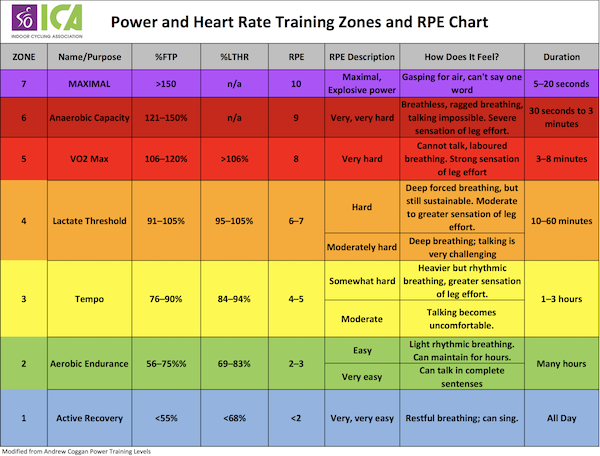
\includegraphics[width=0.6\textwidth]{zones.png}
\end{center}

\paragraph{Sean Hurley: "Normalized Power: What It Is and How to Use It" https://www.trainerroad.com/blog/normalized-power-what-it-is-and-how-to-use-it/}
TrainerRoad writer Sean Hurley provides a useful and consise definition of Normalized Power (NP), a metric invented by Dr. Andrew Coggan in his book \textit{Training and Racing With a Power Meter}. NP
"reflects the disproportionate metabolic cost of riding at high intensity, by weighting hard efforts and deemphasizing periods of easy spinning", according to Dr Coggan.
Essentially, NP approximates what power a rider could have put out for the same effort, if their effort was steady-state. While it is not a completely accurate metric for effort, it is a really
good indication of power variability, and as such is useful in determining the type of effort of a segment. The algorithm for determining NP is as follows:
\begin{enumerate}
	\item Calculate a rolling 30 second average power for the duration
	\item Raise each rolling average value to the fourth power.
	\item Determine the average of all the rolling values
	\item Take the fourth root.
\end{enumerate}

What follows is a formalization of this algorithm.

Let the input power series be:
\[
	P[t], t \in \;[0,T\;]
\]
where $t$ is the time in seconds, and $T$ is the duration of the segment.

Instead of a 30 second rolling average, we will take the lesser of either 30 seconds, or the remaining duration of the segment, so we don't end up
with a lot of segments with skewed NP due to the rolling window running off the edge of the data set.

We will define a variable $k$ that represents this:
\[
	k[t] = \begin{cases}
		(T-t), & (T-t) < 30   \\
		30,    & (T-t) \ge 30 \\
	\end{cases}
\]
Now we can define the rolling average at time $t$ to be:
\[
	\overline{P}_{k[t]}[t] = \frac{1}{k[t]} \sum_{j=0}^{k[t]-1} P[j]

\]
\subsection{Applications in Training Suitability Scoring}

The application of Wavelet analysis in GPX data is a novel and flexible way of determing suitability, as it is a generic signal analysis method. Considering GPX files can
contain multiple signals, Wavelets can be applied to any discrete signal that utilizes numerical reporting. Such signals may include Power, Speed, Cadence, Heart Rate, Elevation, and Heading.


\subsection{Methodological Considerations and Assumptions}

\end{document}
